\documentclass[11pt,a4paper]{article}

\usepackage[margin=1in]{geometry}
\usepackage[T1]{fontenc}
\usepackage{lmodern}
\usepackage{microtype}
\usepackage{array}
\usepackage{booktabs}
\usepackage{longtable}
\usepackage{tabularx}
\usepackage{ragged2e}
\usepackage{enumitem}
\usepackage{xcolor}
\usepackage{hyperref}
\usepackage{graphicx}
\usepackage{tikz}
\usepackage{pdflscape}
\usepackage{fancyhdr}
\usepackage{caption}
\usepackage{amssymb}

\usetikzlibrary{arrows.meta,positioning,fit,shapes.geometric,calc,backgrounds}

\definecolor{ink}{HTML}{17252A}
\definecolor{teal}{HTML}{147D78}
\definecolor{teallight}{HTML}{E8F4F2}
\definecolor{gold}{HTML}{B47719}
\definecolor{goldlight}{HTML}{FFF4DE}
\definecolor{red}{HTML}{A23B3B}
\definecolor{grayline}{HTML}{C9D2D3}

\hypersetup{
  colorlinks=true,
  linkcolor=teal,
  urlcolor=teal,
  citecolor=teal,
  pdftitle={Explainable Privacy-Preserving Multi-Agent Framework for Autonomous Healthcare Software Development},
  pdfauthor={SEM 9 Research Study}
}

\setlist[itemize]{leftmargin=1.35em,itemsep=0.25em}
\setlist[enumerate]{leftmargin=1.55em,itemsep=0.35em}
\renewcommand{\arraystretch}{1.18}
\newcolumntype{L}[1]{>{\RaggedRight\arraybackslash}p{#1}}
\newcolumntype{Y}{>{\RaggedRight\arraybackslash}X}

\pagestyle{fancy}
\fancyhf{}
\fancyhead[L]{\small Explainable Privacy-Preserving Healthcare MAS}
\fancyhead[R]{\small Scoping Literature Study}
\fancyfoot[C]{\thepage}
\setlength{\headheight}{14pt}

\title{\textbf{Explainable Privacy-Preserving Multi-Agent Framework for Autonomous Healthcare Software Development}\\[0.45em]
\large A Scoping Literature Study}
\author{SEM 9 Research Study}
\date{July 2026}

\begin{document}

\maketitle
\thispagestyle{empty}

\begin{abstract}
Healthcare multi-agent systems coordinate specialized components for clinical decision support, patient monitoring, operations, and electronic health record interaction. Their autonomy can improve task decomposition and responsiveness, but it also enlarges the privacy, explanation, and accountability problem. This scoping literature study examines how selected research treats those concerns and asks whether healthcare agents that deliver services can inform agents that build healthcare software. The reviewed literature spans 2018 to 2026 and includes systematic reviews, domain overviews, ethical analysis, and technical prototypes. The purposive scope supports a focused research agenda rather than a claim of exhaustive systematic coverage. A structured evidence matrix records each study's architecture, privacy controls, explanation approach, interoperability support, governance, software-development coverage, evaluation method, limitations, and evidence confidence. Thematic synthesis shows that the strongest concrete mechanisms concern access control, secure communication, FHIR-aware record interaction, encryption, and audit logging. Explainability appears more often as a requirement than as an evaluated mechanism. Reviews also report limited clinical validation, inconsistent metrics, and unresolved responsibility across interacting agents. No included study presents an autonomous, governed software-development lifecycle for healthcare. The study derives a research agenda and proposes a Design Science Research methodology for a framework that assigns specialized agents to requirements, compliance, architecture, coding, privacy, explanation, testing, clinical safety, and provenance. The proposed evaluation compares a single agent, an uncontrolled multi-agent workflow, and the full governed framework using synthetic FHIR data. The resulting contribution is positioned as healthcare software engineering under privacy, explanation, interoperability, and human-approval constraints, not as another clinical chatbot or decision-support agent.
\end{abstract}

\noindent\textbf{Keywords:} multi-agent systems; agentic AI; healthcare software engineering; privacy by design; explainable AI; FHIR; provenance; Design Science Research

\clearpage
\tableofcontents
\clearpage

\section{Introduction and Scope}

\subsection{Motivation}

Healthcare software sits inside a dense network of clinical, technical, and institutional constraints. A system may need to exchange records across organizational boundaries, restrict access by role and purpose, preserve an audit trail, represent consent, support clinical review, and recover safely when a component fails. These obligations apply before a model produces a diagnosis or a scheduling recommendation. They shape requirements, architecture, code, tests, configuration, deployment, and maintenance. Software-development automation in this setting therefore carries a different risk profile from general code generation.

Multi-agent systems (MAS) offer a plausible way to divide this work. A team can assign separate responsibilities to agents that interpret requirements, design services, generate code, inspect privacy risks, test security controls, or record provenance. The same division creates new failure paths. One agent can disclose sensitive context to another, accept a fabricated result, exceed its authority, or produce an explanation that does not match the action it took. A final artifact may combine decisions from several agents, making responsibility difficult to reconstruct. Xie et al. describe closely related problems in clinical MAS as compound opacity, error propagation, attribution difficulty, automation bias, erosion of human oversight, privacy risk, consent threats, and contextual blindness \cite[pp.~5--12]{xie2026ethical}. Those risks transfer to software artifacts even when the agents never make a direct clinical decision.

The available healthcare MAS literature does not begin from software development. Earlier work reviewed scheduling, routing, and resource allocation in home healthcare \cite{becker2018survey}. Recent studies examine clinical AI agents, decision support, robotic interventions, critical care, record access, multilingual interaction, and ethical governance \cite{gorenshtein2025clinical,ode2025evidence,demaio2025privacy,shehab2025agentic}. These studies provide architectural and governance lessons, but the transfer from service-delivery agents to software-building agents needs explicit analysis. A privacy mechanism that protects an EHR query, for example, does not automatically protect prompts, generated test fixtures, tool traces, agent memory, source code, or deployment logs.

This chapter studies that transfer. It maps mechanisms and limitations across the reviewed literature, identifies findings supported with reasonable confidence, and marks claims that remain uncertain because the scope is narrow. It then converts the supported gaps into requirements for a future explainable, privacy-preserving multi-agent software-engineering framework.

\subsection{Aim and objectives}

The study aims to determine how current healthcare MAS research can inform a governed framework for autonomous healthcare software development. Five objectives guide the analysis:

\begin{enumerate}
  \item classify the agent architectures, healthcare settings, and autonomy patterns represented in the corpus;
  \item identify concrete privacy, security, explanation, interoperability, and governance mechanisms;
  \item assess how authors validate their systems and where the evidence remains weak;
  \item determine which software-development lifecycle activities the papers address directly; and
  \item derive a traceable research methodology and evaluation plan for the proposed framework.
\end{enumerate}

The chapter does not estimate a pooled clinical effect. The included studies differ in purpose, design, outcome, and unit of analysis. Some are technical prototypes, some are systematic reviews of other studies, and others are narrative or ethical reviews. A meta-analysis would combine unlike evidence and give false precision. The study instead uses descriptive classification and thematic synthesis.

\subsection{Review questions}

Six review questions connect the literature study to the proposed research:

\begin{description}[leftmargin=3.6em,style=nextline]
  \item[RQ1] Which architectural patterns and forms of coordination appear in healthcare multi-agent systems?
  \item[RQ2] How do the included studies implement or discuss privacy, security, explainability, interoperability, and governance?
  \item[RQ3] How strong is the reported validation, and which limits affect transfer to regulated software engineering?
  \item[RQ4] Which healthcare software-development lifecycle activities receive direct support in the corpus?
  \item[RQ5] Which research gaps support a governed, explainable, privacy-preserving development framework?
  \item[RQ6] How should future research build and evaluate that framework without using real patient data?
\end{description}

\subsection{Boundary of the claim}

The review concentrates on healthcare MAS, agentic AI, privacy, security, explainability, interoperability, and ethics. It uses purposive selection tied to the review questions rather than an exhaustive database search. This boundary allows the chapter to establish what the included literature covers and omits, but it cannot establish that no relevant work exists outside the review scope.

This distinction matters most for the proposed novelty claim. No included study presents an autonomous healthcare software-development framework. That is a review-supported observation. The stronger statement that no such framework exists anywhere is a scope-boundary hypothesis. A later systematic search across software engineering, secure software development, medical-device engineering, and agentic coding research would need to test it.

\section{Conceptual Foundations}

\subsection{Multi-agent systems and agentic AI}

A software agent perceives information, applies a decision process, and acts toward an assigned objective. A multi-agent system combines agents that communicate or coordinate while retaining distinct roles or state. In classical healthcare MAS, an agent may represent a patient, clinician, scheduler, care resource, sensor, or institutional service. Becker et al. found these abstractions in home-care routing and scheduling, where agents support decentralized planning and simulation \cite[pp.~5--10]{becker2018survey}. Naresh et al. use a layered smart-city model in which healthcare stakeholders exchange protected group information through agent-mediated communication \cite[pp.~3--9]{naresh2020quantum}.

Agentic AI built on large language models adds tool use, iterative planning, memory, and natural-language coordination. Gorenshtein et al. define a clinical AI agent through iterative reasoning plus tool selection or multi-agent collaboration; their stricter multi-agent category requires iterative reasoning and collaboration \cite[pp.~23--24]{gorenshtein2025clinical}. Their review identifies three broad patterns: a single agent that calls tools, multiple agents without tool integration, and a hybrid architecture that combines both. These categories help separate a prompted model from a system that can decompose and execute a workflow.

Autonomy is not a binary property. An agent may recommend an action, execute it inside a sandbox, modify an external record, or deploy a generated service. The risk rises with action authority, persistence, and difficulty of reversal. De Maio et al. make this distinction concrete by routing record retrieval and record updates through different paths and a dedicated Data Update Agent \cite[pp.~3--6]{demaio2025privacy}. A software-development framework needs similar boundaries: reading a requirement, editing code, approving a migration, and deploying to production should not share one permission level.

\subsection{Privacy preservation as a lifecycle property}

Healthcare privacy involves more than encryption. A system must limit collection, restrict access, preserve purpose, control disclosure, record use, and support review. The corpus offers several mechanisms at different layers. Khan and Reyad assign authentication, authorization, and record-sharing responsibilities to access-control agents \cite[pp.~2--5]{khan2019ibac}. Naresh et al. protect group communication through a dynamic quantum group-key agreement protocol \cite[pp.~9--20]{naresh2020quantum}. Shehab combines role-based access control, AES-GCM field encryption, and tamper-evident audit logging in a prototype compliance layer \cite[pp.~2--4]{shehab2025agentic}. De Maio et al. control retrieval and updates to FHIR-based records through a modular LLM-agent architecture \cite[pp.~3--8]{demaio2025privacy}.

These mechanisms address runtime health information. Autonomous development introduces additional data surfaces. Requirements can contain patient examples. Prompts can expose business rules, credentials, or system architecture. Agent memory can retain information after a task ends. Tool output can place health data in logs. Generated tests can reproduce identifiable records. Code review traces can reveal vulnerabilities. Privacy by design for development agents must therefore govern data before, during, and after generation. It must also separate data needed to build a feature from data needed to run it.

Privacy and security overlap but answer different questions. Security asks whether unauthorized actors can alter, observe, or disrupt the system. Privacy asks whether any actor, including an authorized one, uses personal information for a justified and limited purpose. An encrypted prompt can still violate minimization. A correct access-control rule can still expose more fields than a test requires. The proposed framework must evaluate both properties rather than treating encryption as proof of privacy.

\subsection{Explainability for decisions and artifacts}

Healthcare explainability research often focuses on a model output: why a system suggested a diagnosis, risk level, or treatment. The included reviews repeatedly identify transparency as a condition for trust and adoption \cite{ode2025evidence,saeed2025applications,boye2025decision}. Shehab demonstrates natural-language diagnostic reasoning in a multilingual prototype, but does not evaluate whether the explanation faithfully reflects the model's internal process \cite[pp.~1--4]{shehab2025agentic}. Xie et al. show why a multi-agent setting makes the problem harder: several locally plausible actions can produce a global result whose cause no participant can reconstruct \cite[pp.~5--8]{xie2026ethical}.

Software artifacts need a different explanation contract. A requirement explanation should identify the source statement, interpretation, assumptions, and affected privacy obligations. An architecture explanation should state alternatives, rejected options, data flows, and trust boundaries. A code explanation should link a change to a requirement and describe security-relevant behavior. A test explanation should state which risk or requirement the test covers and what a failure means. A deployment explanation should show evidence, approvals, unresolved risks, and rollback conditions.

An explanation also serves different readers. A developer needs implementation rationale. A privacy reviewer needs data lineage and purpose. A clinician needs the effect on workflow and patient safety. An auditor needs provenance and approval history. One generic chain-of-thought narrative cannot satisfy these roles and may expose sensitive information. The framework should generate structured, role-appropriate explanations from recorded evidence, not disclose hidden reasoning or produce unconstrained post hoc prose.

\subsection{Healthcare interoperability}

Interoperability determines whether software can exchange and interpret health information across systems. FHIR provides a resource-oriented basis for healthcare APIs, while related standards and terminologies support messaging, imaging, clinical concepts, and audit events. In the corpus, De Maio et al. offer the clearest standards-based implementation: agents map natural-language interaction to FHIR-aware record retrieval and update operations \cite[pp.~1--8]{demaio2025privacy}. Their future work names DICOM and HL7 extensions, which signals that one standard does not cover every exchange need.

Other papers discuss EHR integration more generally. Khan and Reyad focus on access to shared EHR repositories \cite{khan2019ibac}. The reviews by Saeed et al., Okeke et al., and Boye et al. describe fragmented records and legacy integration as adoption barriers \cite{saeed2025applications,okeke2025overview,boye2025decision}. The evidence supports FHIR as a useful technical anchor, but not as a complete compliance solution. A syntactically valid resource can still disclose the wrong information, omit consent constraints, or encode an unsafe workflow.

For autonomous development, interoperability must become executable evidence. Agents should generate resources, profiles, API contracts, and synthetic fixtures that validators can check. They should link each generated interface to access-control rules, audit expectations, and tests. This approach makes standards conformance measurable instead of leaving it as a design claim.

\subsection{Autonomous healthcare software development}

Autonomous software development refers here to agents that perform a bounded portion of the software lifecycle: interpret requirements, propose architecture, generate or modify code, create tests, inspect risks, produce documentation, and prepare deployment evidence. Autonomy does not imply unsupervised production deployment. High-risk transitions can require human approval, and agents can work inside sandboxes with restricted tools.

None of the included studies defines this lifecycle. De Maio et al. and Shehab describe software architectures, while Becker et al. assess implementation availability in prior systems \cite{demaio2025privacy,shehab2025agentic,becker2018survey}. These studies concern the construction or review of agent systems, not systems in which agents build healthcare software. The proposed research therefore transfers mechanisms from the literature into a new unit of analysis: the generated artifact and its lineage.

\subsection{Provenance, accountability, and human governance}

Provenance records where an artifact came from, who or what changed it, which inputs and policies influenced the change, and which evidence supported approval. Accountability assigns responsibility for reviewing, accepting, rejecting, or correcting that artifact. Audit logs contribute to provenance, but an event log alone does not explain why a decision was allowed or who owned the final risk.

The corpus exposes this gap from two directions. Shehab makes tamper-evident logging a first-class control \cite[pp.~2--4]{shehab2025agentic}. Xie et al. show that distributed decision-making blurs responsibility and can reduce human oversight to a procedural approval \cite[pp.~6--11]{xie2026ethical}. A development framework must connect these concerns. Each artifact should carry a machine-readable lineage from requirement to change, test, review, and approval. Human gates must have enough evidence and authority to stop the workflow. A record of a click is not meaningful oversight if the reviewer cannot inspect the relevant risk.

\section{Scoping Review Method}

\subsection{Review design}

This study uses a structured scoping design to map concepts, mechanisms, evidence quality, and gaps across selected literature. The method borrows transparent reporting practices from systematic reviews, but it does not label the result a systematic review. Purposive selection follows the review questions and topic boundaries rather than an exhaustive database-search protocol. This design prevents an exhaustive coverage claim.

The method follows six steps: define the scope and review questions, apply relevance criteria, extract evidence into a common matrix, classify and appraise each source, synthesize findings by theme, and derive research gaps and framework requirements. The matrix is stored separately as \texttt{evidence\_matrix.csv}. It records page locations so that claims can be checked against the source publications.

\subsection{Review procedure}

Figure~\ref{fig:workflow} summarizes the review procedure. The sequence keeps the final research gaps traceable to the review questions, extracted evidence, and quality appraisal.

\begin{figure}[htbp]
\centering
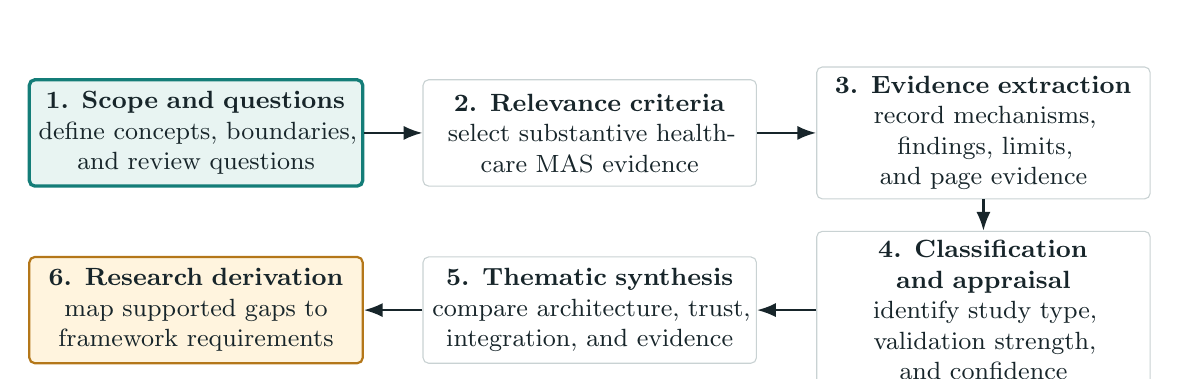
\begin{tikzpicture}[
  stage/.style={draw=grayline,rounded corners=2pt,fill=white,text width=4cm,
    minimum height=1.35cm,align=center,text=ink,font=\small},
  primary/.style={stage,draw=teal,fill=teallight,very thick},
  outcome/.style={stage,draw=gold,fill=goldlight,thick},
  arrow/.style={-{Latex[length=2.4mm]},thick,draw=ink}
]
\node[primary] (scope) at (-5,0) {\textbf{1. Scope and questions}\\define concepts, boundaries, and review questions};
\node[stage] (eligibility) at (0,0) {\textbf{2. Relevance criteria}\\select substantive healthcare MAS evidence};
\node[stage] (extract) at (5,0) {\textbf{3. Evidence extraction}\\record mechanisms, findings, limits, and page evidence};
\node[stage] (appraise) at (5,-2.25) {\textbf{4. Classification and appraisal}\\identify study type, validation strength, and confidence};
\node[stage] (synthesis) at (0,-2.25) {\textbf{5. Thematic synthesis}\\compare architecture, trust, integration, and evidence};
\node[outcome] (gaps) at (-5,-2.25) {\textbf{6. Research derivation}\\map supported gaps to framework requirements};
\draw[arrow] (scope) -- (eligibility);
\draw[arrow] (eligibility) -- (extract);
\draw[arrow] (extract) -- (appraise);
\draw[arrow] (appraise) -- (synthesis);
\draw[arrow] (synthesis) -- (gaps);
\end{tikzpicture}
\caption{Scoping-review workflow used to connect the research questions, evidence synthesis, and proposed framework requirements.}
\label{fig:workflow}
\end{figure}

Bibliographic identity, publication status, and study type were checked before extraction. The evidence matrix uses verified titles, authors, years, and publication details so that similar studies remain distinct during synthesis.

\subsection{Eligibility criteria}

A study qualified for inclusion when it was written in English, addressed healthcare or e-health, and made a substantive contribution to MAS architecture, agentic AI, privacy, security, explainability, EHR/FHIR interaction, evaluation, or governance. Publication status did not determine inclusion because the review maps concepts and mechanisms across different forms of evidence. The appraisal records peer-review and preprint status so that readers can weight claims accordingly.

The review excluded studies outside the healthcare context and sources that did not provide enough substantive evidence for the review questions. Negative findings and weak validation remained eligible because they help identify limitations and research gaps.

\subsection{Data extraction}

The extraction form covered bibliographic identity, study type, objective, healthcare setting, agent architecture, autonomy, privacy and security, explainability, interoperability, governance, human oversight, software-development coverage, evaluation, data, findings, limitations, page evidence, and quality categories. Keyword searching supported navigation, but keyword counts did not determine themes. A page containing the word ``privacy'' may only cite related work. Each coded mechanism therefore required contextual reading.

The extraction also distinguishes direct evidence from recommendations. A prototype that implements RBAC provides direct architectural evidence. A narrative review that recommends privacy by design provides evidence that scholars recognize the need, not evidence that a control works. This distinction limits double-counting because several 2025 reviews discuss overlapping source studies.

\subsection{Study classification and quality appraisal}

The included literature was classified as systematic reviews, narrative reviews, conceptual or ethical analyses, and technical prototypes or protocols. A categorical appraisal replaced a numerical score. Different study types cannot be ranked fairly on one scale: a cryptographic protocol and an ethical review answer different questions.

Five categories were recorded. \emph{Publication status} identifies peer review or preprint status. \emph{Method transparency} asks whether the paper explains selection, architecture, data, and analysis. \emph{Topic relevance} measures contribution to the combined privacy, explanation, MAS, and healthcare-software problem. \emph{Validation strength} considers implementation, comparison, realistic data, and deployment. \emph{Reproducibility} considers whether another researcher could reconstruct the study from the reported method and artifacts. The final evidence-confidence label summarizes judgment as high, medium, or low without implying a validated measurement scale.

\subsection{Synthesis method}

The analysis began with deductive themes taken from the review questions: architecture, privacy, explainability, interoperability, governance, validation, and software-development coverage. Inductive coding then captured recurring concerns such as modularity, error propagation, legacy integration, auditability, agent authentication, and missing real-world trials. Figure~\ref{fig:taxonomy} shows the resulting taxonomy.

\begin{figure}[htbp]
\centering
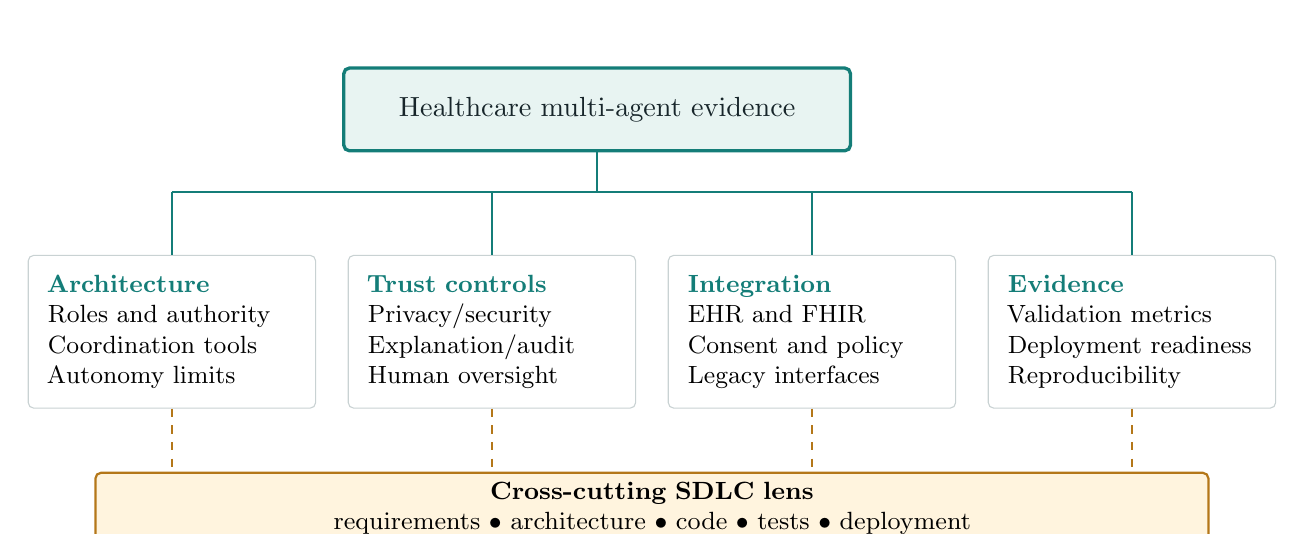
\begin{tikzpicture}[
  root/.style={draw=teal,fill=teallight,very thick,rounded corners=2pt,
    align=center,text width=6.2cm,minimum height=1.05cm,text=ink},
  theme/.style={draw=grayline,fill=white,rounded corners=2pt,align=left,
    text width=3.15cm,minimum height=1.75cm,font=\small,inner sep=2.5mm},
  cross/.style={draw=gold,fill=goldlight,thick,rounded corners=2pt,align=center,
    text width=13.9cm,minimum height=0.9cm,font=\small},
  edge/.style={draw=teal,thick},
  crossedge/.style={draw=gold,thick,dashed}
]
\node[root] (root) {Healthcare multi-agent evidence};
\node[theme,below=13mm of root,xshift=-5.4cm] (arch)
  {\textbf{\color{teal}Architecture}\\Roles and authority\\Coordination tools\\Autonomy limits};
\node[theme,right=4mm of arch] (trust)
  {\textbf{\color{teal}Trust controls}\\Privacy/security\\Explanation/audit\\Human oversight};
\node[theme,right=4mm of trust] (integration)
  {\textbf{\color{teal}Integration}\\EHR and FHIR\\Consent and policy\\Legacy interfaces};
\node[theme,right=4mm of integration] (evidence)
  {\textbf{\color{teal}Evidence}\\Validation metrics\\Deployment readiness\\Reproducibility};
\coordinate (split) at ($(root.south)+(0,-5mm)$);
\draw[edge] (root.south) -- (split);
\draw[edge] (arch.north |- split) -- (evidence.north |- split);
\foreach \x in {arch,trust,integration,evidence}
  \draw[edge] (\x.north |- split) -- (\x.north);
\coordinate (midcards) at ($(trust.south)!0.5!(integration.south)$);
\node[cross,below=8mm of midcards] (sdlc)
  {\textbf{Cross-cutting SDLC lens}\\
   requirements \(\bullet\) architecture \(\bullet\) code \(\bullet\) tests \(\bullet\) deployment};
\foreach \x in {arch,trust,integration,evidence}
  \draw[crossedge] (\x.south) -- (\x.south |- sdlc.north);
\end{tikzpicture}
\caption{Taxonomy used for thematic synthesis. Software-development coverage was assessed across all four branches.}
\label{fig:taxonomy}
\end{figure}

The synthesis compares patterns rather than pooling outcomes. Quantitative figures reported by review papers are treated as secondary claims. The chapter does not add sample sizes across reviews because their included studies may overlap. Strong conclusions require convergence across source types or a direct mechanism supported by implementation evidence.

\subsection{Threats to validity}

Selection bias is the largest threat. The purposive scope emphasizes healthcare MAS and gives less attention to software engineering, medical-device engineering, and agentic coding. Publication dates also cluster in 2025, which can overrepresent current LLM-agent terminology and underrepresent earlier software-agent engineering.

Extraction carries interpretive risk. The papers use ``agent,'' ``agentic AI,'' and ``multi-agent'' inconsistently. The matrix records the architecture described by each author, but this chapter applies Gorenshtein et al.'s distinction when comparing systems \cite[pp.~23--24]{gorenshtein2025clinical}. Page references follow the pagination shown in each source publication, which may differ from printed journal numbers.

Evidence quality varies. Broad reviews in lower-visibility venues report ambitious benefits while providing limited traceability to primary outcomes. A preprint review has a stronger registered method but has not completed peer review. Technical prototypes demonstrate feasibility but not clinical safety. The synthesis addresses these differences through confidence labels and cautious wording.

\section{Background Study}

The background study compares the reviewed work by publication context, research focus, reported findings, and technical approach. Table~\ref{tab:background-study} provides a structural overview before the thematic synthesis. The table is descriptive: a listed mechanism indicates that a study implemented or substantively discussed it, not that the mechanism has been clinically validated or shown superior to alternatives.

\begingroup
\hypersetup{citecolor=black,linkcolor=black}
\setlength{\tabcolsep}{2.5pt}
\renewcommand{\arraystretch}{1.08}
\footnotesize
\begin{longtable}{|L{0.65cm}|L{1.85cm}|L{1.90cm}|L{3.10cm}|L{3.80cm}|L{2.90cm}|}
\caption{Structural overview of the background literature.}\label{tab:background-study}\\
\hline
\textbf{ID} & \textbf{Authors} & \textbf{Venue and year} & \textbf{Study title} & \textbf{Key observations} & \textbf{Methods and technologies} \\
\hline
\endfirsthead
\multicolumn{6}{c}{\footnotesize\textit{Table~\thetable\ continued from the previous page}}\\
\hline
\textbf{ID} & \textbf{Authors} & \textbf{Venue and year} & \textbf{Study title} & \textbf{Key observations} & \textbf{Methods and technologies} \\
\hline
\endhead
\hline
\multicolumn{6}{r}{\footnotesize\textit{Continued on the next page}}\\
\endfoot
\hline
\endlastfoot
S01 & Becker et al. & MATES/\allowbreak CEUR, 2018 & Survey of Multiagent Systems for Improving Home Health Care Management \cite{becker2018survey} & Healthcare MAS support decentralized planning and simulation, but the reviewed approaches lacked the implementation and evaluation maturity required for practical use. & Systematic literature review; home-care routing, scheduling, resource allocation, and agent-based simulation. \\
\hline
S02 & Khan and Reyad & Information Sciences Letters, 2019 & Application of Intelligent Multi Agent Based Systems for E-Healthcare Security \cite{khan2019ibac} & Separating authentication, authorization, and record-sharing responsibilities across agents offers a conceptual security architecture, but the model lacks implementation and measured accuracy. & Agent-mediated EHR access control; authentication, authorization, confidentiality, and controlled record sharing. \\
\hline
S03 & Naresh et al. & Sensors, 2020 & Quantum Diffie--Hellman Extended to Dynamic Quantum Group Key Agreement for e-Healthcare Multi-Agent Systems in Smart Cities \cite{naresh2020quantum} & The protocol provides a specialized confidentiality mechanism for dynamic healthcare-agent groups and analyzes join, leave, internal, and external attack cases. & Dynamic quantum group-key agreement; controller-based healthcare MAS; protocol-efficiency and attack analysis. \\
\hline
S04 & De Maio et al. & JCSS, 2025 & Privacy-Preserving Healthcare Data Interactions: A Multi-Agent Approach Using LLMs \cite{demaio2025privacy} & A modular LLM-agent architecture demonstrates controlled retrieval and update of interoperable health records, providing the strongest direct bridge between agents, privacy, and FHIR. & LLM specialist agents; policy-aware routing; FHIR retrieval and update paths; scenario, robustness, and scalability tests. \\
\hline
S05 & Shehab & arXiv, 2025 & Agentic-AI Healthcare: Multilingual, Privacy-First Framework with MCP Agents \cite{shehab2025agentic} & Privacy controls and orchestrated specialist agents coexist in one prototype, although explanation faithfulness and comparative validation remain untested. & MCP orchestration; symptom, medication, and appointment agents; RBAC; AES-GCM; tamper-evident audit logging. \\
\hline
S06 & Gorenshtein et al. & medRxiv, 2025 & AI Agents in Clinical Medicine: A Systematic Review \cite{gorenshtein2025clinical} & Clinical-agent architectures can improve base-model performance when matched to task complexity, but safety evidence, explainability analysis, and prospective validation remain limited. & Systematic review; single-agent tool use, multi-agent collaboration, hybrid architectures, QUADAS-AI appraisal. \\
\hline
S07 & Ode et al. & IJLTEMAS, 2025 & Multi-Agent AI Systems in Healthcare: Systematic Evidence Synthesis Via PRISMA \cite{ode2025evidence} & MAS show potential in decision support, robotics, and critical care, while clinical validation and treatment of ethical or legal issues remain uneven. & PRISMA-style systematic synthesis; BDI, fuzzy, reinforcement-learning, modular specialist, and robotic architectures. \\
\hline
S08 & Saeed et al. & IJSDR, 2025 & Multi-agent Artificial Intelligence Systems in Health Care: Applications, Challenges, and Future Prospects \cite{saeed2025applications} & Adoption depends on trust, interoperability, privacy, explainability, and governance, but the paper treats these controls primarily at a narrative level. & Narrative review; EHR integration, encryption, federated learning, access control, and healthcare coordination. \\
\hline
S09 & Okeke et al. & IJSDR, 2025 & Multiagent AI Systems in Healthcare: An Overview of Its Applications in Aspects of Healthcare \cite{okeke2025overview} & Distributed agents can coordinate care tasks, but fragmented records, legacy integration, privacy risk, and governance constrain adoption. & Narrative overview; healthcare coordination, decision support, monitoring, logistics, and EHR integration challenges. \\
\hline
S10 & Boye et al. & IJSDR, 2025 & Multiagent Artificial Intelligence Systems for Decision Support in Healthcare: A Systematic Review \cite{boye2025decision} & MAS support complex decision-making, although the evidence remains fragmented and explanation, integration, validation, and responsibility need stronger treatment. & Systematic review of decision-support MAS; comparative study selection and qualitative synthesis. \\
\hline
S11 & Xie et al. & Frontiers in Public Health, 2026 & Ethical Issues in Multi-Agent AI Systems for Healthcare: A Narrative Review \cite{xie2026ethical} & Distributed decision-making creates compound opacity, cascading error, attribution difficulty, consent risks, and potential erosion of clinician authority. & Ethical narrative review; accountability, privacy-centered design, adaptive governance, explanation, and human oversight. \\
\hline
S12 & Yusuf et al. & IJCMS, 2025 & A Systematic Review of Multi-Agent Systems in Healthcare \cite{yusuf2025systematic} & MAS offer clinical and operational benefits, but interoperability, regulatory compliance, privacy, stakeholder readiness, and accountability remain adoption barriers. & Systematic review; privacy by design, blockchain, federated learning, EHR integration, and strategic adoption measures. \\
\end{longtable}
\endgroup

\subsection{Synthesis of Prior Work}

\subsubsection{Publication period and study types}

The reviewed literature spans 2018 to 2026, with most publications appearing in 2025 or 2026. This concentration reflects the rise of LLM-based agents. The older studies cover classical software agents, access control, and secure communication; the recent studies add tool-using LLMs, MCP orchestration, FHIR interaction, and agent ethics.

The sources include systematic reviews or studies with systematic search methods \cite{becker2018survey,gorenshtein2025clinical,ode2025evidence,boye2025decision,yusuf2025systematic}, narrative and domain overviews \cite{saeed2025applications,okeke2025overview,xie2026ethical}, and proposed models, protocols, or prototypes \cite{khan2019ibac,naresh2020quantum,demaio2025privacy,shehab2025agentic}. This mixture supports concept mapping but does not establish whether one architecture outperforms another.

\subsubsection{Application coverage}

The studies cover home-care scheduling, EHR access, smart-city communication, clinical record interaction, symptom and medication support, diagnosis, evidence synthesis, treatment planning, robotics, critical care, logistics, monitoring, and ethics. Decision support dominates the reviews. Gorenshtein et al. report diagnosis and prognosis as the largest category in their 20 included studies, followed by evidence synthesis and treatment planning \cite[pp.~10--12]{gorenshtein2025clinical}. Ode et al. divide 32 studies among clinical decision support, robotic interventions, and critical care \cite[pp.~1--4]{ode2025evidence}.

No paper evaluates agents whose primary product is healthcare software. Some papers describe architectures or implementations, but their agents serve patients, clinicians, or data workflows. This absence becomes the central bridge to the proposed research.

\subsubsection{Evidence maturity}

The corpus contains concrete technical work but little deployment evidence. Becker et al. found no reviewed home-care approach suitable for practical application because implementation provision and evaluation were weak \cite[pp.~11--12]{becker2018survey}. Khan and Reyad leave real-time implementation and accuracy evaluation to future work \cite[p.~5]{khan2019ibac}. De Maio et al. run scenario and robustness evaluations, yet still call for testing in real healthcare environments \cite[pp.~6--9]{demaio2025privacy}. Shehab labels the system a research prototype and not a certified medical device \cite[p.~1]{shehab2025agentic}.

The reviews reach the same conclusion at a broader scale. Ode et al. report that more than 60 percent of included studies lacked clinical validation \cite[p.~1]{ode2025evidence}. Gorenshtein et al. find only six of 20 studies at low risk of bias across all QUADAS-AI domains and only one prospective randomized trial \cite[pp.~10--13]{gorenshtein2025clinical}. The evidence supports feasibility and research direction more strongly than routine clinical readiness.

\subsubsection{Architectures and coordination patterns}

The corpus shows a progression from domain-representative agents to LLM-based specialist teams. Classical MAS assign agents to stable entities or functions. Home-care systems model caregivers, patients, schedules, and resources to optimize routing and allocation \cite{becker2018survey}. Khan and Reyad divide EHR security into agent responsibilities for access and sharing \cite{khan2019ibac}. Naresh et al. organize communication by geographic zone and use a controller to construct a group key \cite{naresh2020quantum}.

Recent systems assign cognitive or workflow roles. De Maio et al. distinguish query interpretation, data retrieval, and data update, then route a request through the appropriate path \cite[pp.~3--6]{demaio2025privacy}. Shehab uses symptom, medication, and appointment agents under MCP orchestration \cite[pp.~2--4]{shehab2025agentic}. These designs illustrate two useful principles for software development: separate privileges by task, and place routing logic at a governed boundary.

The review evidence shows no dominant architecture. Gorenshtein et al. classify eight of 20 clinical studies as single-agent tool-calling, five as multi-agent without tools, and seven as hybrid systems \cite[pp.~10--12]{gorenshtein2025clinical}. Ode et al. report BDI, fuzzy-logic, reinforcement-learning, modular specialist, and robotic architectures \cite[pp.~3--6]{ode2025evidence}. Architectural choice follows task structure rather than a universal template.

This finding argues against creating many agents for its own sake. A future framework should assign an agent only when the role needs distinct tools, permissions, expertise, or independent review. Otherwise, additional communication increases latency and creates another failure surface. The architecture should also record whether an agent recommends, modifies, approves, or executes. Those verbs imply different authority.

Coordination mechanisms receive less evaluation than end-task performance. Studies often report that agents collaborate, but they do not measure message integrity, conflict resolution, deadlock, stale state, or the effect of a faulty agent. Xie et al.'s error-propagation concern therefore has limited empirical treatment in the technical corpus \cite[pp.~5--7]{xie2026ethical}. A software-development experiment should inject faulty and malicious messages rather than assume cooperative agents.

\subsubsection{Privacy, security, and data governance}

Privacy appears throughout the literature, but implemented controls concentrate in work by Khan and Reyad, Naresh et al., De Maio et al., and Shehab. Khan and Reyad propose agent-based EHR access control \cite{khan2019ibac}. Naresh et al. contribute secure group-key agreement for communicating healthcare agents \cite{naresh2020quantum}. De Maio et al. constrain FHIR retrieval and update workflows \cite{demaio2025privacy}. Shehab integrates RBAC, field encryption, and audit logging \cite{shehab2025agentic}. Together they cover authorization, confidentiality in transit or storage, controlled modification, and auditability.

The controls remain isolated. The access-control proposal lacks implementation. The quantum protocol secures communication but does not determine whether the data should have been shared. The FHIR framework governs record operations but does not address software-generation traces. The MCP prototype combines several controls, yet provides illustrative rather than comparative evaluation. No paper supplies an end-to-end privacy model spanning input collection, agent memory, inter-agent messages, tool calls, generated artifacts, logs, retention, and deletion.

Narrative and systematic reviews broaden the list of concerns. Saeed et al. discuss encryption, federated learning, privacy, and regulatory barriers \cite[pp.~7--12]{saeed2025applications}. Yusuf et al. identify privacy by design, blockchain, and federated learning as strategic responses \cite[pp.~6--9]{yusuf2025systematic}. Ode et al. find that only a minority of reviewed studies address ethical and legal implications in depth \cite[pp.~4--7]{ode2025evidence}. These sources support the importance of privacy, but they do not establish which mechanism works best.

For development agents, the missing control plane matters more than any individual cryptographic choice. The framework needs data classification before an agent receives context; least-privilege tools during execution; message filtering between agents; isolated memory; redacted logs; synthetic test data; retention limits; and reviewable policy decisions. Encryption should protect permitted data flows. It cannot decide permission by itself.

Consent also receives limited operational treatment. Xie et al. identify opaque recommendations and distributed data use as threats to informed consent and patient autonomy \cite[pp.~8--10]{xie2026ethical}. The technical papers do not show agents reading a machine-actionable consent directive and enforcing it across tasks. A future FHIR-based prototype can turn consent into a testable input: an agent should fail a request when the purpose, role, or resource falls outside the synthetic patient's policy.

\subsubsection{Explainability and transparency}

Explainability has high rhetorical coverage and low measurement maturity. The reviews call for transparent systems that clinicians and patients can trust \cite{ode2025evidence,saeed2025applications,boye2025decision}. Xie et al. give the strongest account of why ordinary explanation methods may fail in MAS. Interacting agents create layers of reasoning and delegation, while attribution becomes harder after an error moves through the chain \cite[pp.~5--8]{xie2026ethical}.

Shehab presents transparent diagnostic reasoning as a prototype feature \cite[pp.~1--4]{shehab2025agentic}. De Maio et al. expose modular routing and controlled data operations, which makes parts of the workflow inspectable \cite[pp.~3--7]{demaio2025privacy}. Neither study evaluates explanation faithfulness, completeness, stability, reader comprehension, or decision impact. No study compares explanation formats across clinicians, developers, privacy officers, and auditors.

The literature also tends to conflate transparency with explanation. A system can publish its architecture while leaving a particular action unexplained. It can log an event without recording rationale. It can generate a fluent rationale that cites no evidence. The proposed framework should separate four artifacts: an event trace, an evidence link, a policy decision, and a reader-facing explanation. Each has a distinct verification method.

Artifact-level explanation is absent. None of the papers defines how an agent should explain a requirement interpretation, architecture choice, source-code change, failed test, accepted risk, or deployment decision. This is not a criticism of studies aimed at clinical service delivery. It is a direct limit on their transfer to autonomous development.

An artifact explanation should remain concise and structured. At minimum, it should include the originating requirement, the agent and model version, tools and data classes used, policy constraints applied, alternatives considered, tests or validators run, unresolved risks, and required approval. This record can support audit without exposing private chain-of-thought content.

\subsubsection{FHIR, EHR, and legacy integration}

The corpus treats EHRs as both a resource and a risk. Khan and Reyad focus on protecting shared records \cite{khan2019ibac}. De Maio et al. make FHIR the interface between natural-language requests and structured retrieval or update operations \cite[pp.~1--8]{demaio2025privacy}. Reviews describe fragmented systems and legacy integration as barriers to adoption \cite{saeed2025applications,okeke2025overview,boye2025decision}.

De Maio et al. provide the strongest implementation anchor for the proposed framework. FHIR resources can support synthetic tasks with machine-checkable structure. A development agent can generate an API endpoint, access rule, audit event, and test fixture around a resource. A validator can then check conformance without exposing real patient information. This creates a reproducible experimental setting.

FHIR alone does not settle semantics or governance. Local profiles, terminology bindings, workflow rules, and institutional policies affect valid use. The framework must therefore treat standards as constraints supplied to agents, not as facts the model can improvise. When a required profile or policy is absent, the system should raise a blocking question or produce a clearly labeled assumption rather than invent a compliant-looking artifact.

Legacy integration remains underdeveloped in the direct evidence. The reviews describe it, but the prototypes do not compare strategies for migration, adapters, or partial failure. A realistic software-development task should include an incompatible or incomplete interface so that architecture and test agents must expose assumptions and degraded behavior.

\subsubsection{Ethics, accountability, and human oversight}

Ethical analysis provides the clearest warning against unrestricted autonomy. Xie et al. identify seven challenge groups and argue for adaptive governance, clear responsibility, preserved clinician authority, explainability, and privacy-centered design \cite[pp.~5--13]{xie2026ethical}. Ode et al. report weak treatment of ethics and law across reviewed implementations \cite[pp.~4--7]{ode2025evidence}. Gorenshtein et al. also call for stronger safety evaluation and real-world trials \cite[pp.~20--24]{gorenshtein2025clinical}.

Human-in-the-loop language does not guarantee control. A reviewer who sees only the final output cannot assess a chain of hidden transformations. Repeated approvals can encourage automation bias, especially when the system usually succeeds. A meaningful gate needs a defined owner, risk threshold, evidence bundle, rejection path, and rollback authority. It should interrupt the workflow before an irreversible action, not ask for confirmation afterward.

Responsibility must attach to organizational roles as well as agents. An audit record can identify which agent generated a migration, but a person or team must own the decision to run it. The framework should therefore distinguish production of evidence from acceptance of risk. Agents can recommend and verify; designated humans approve high-risk transitions.

Patient involvement receives less attention than clinician oversight. Xie et al. connect autonomy and consent to patient rights \cite[pp.~8--10]{xie2026ethical}. A software-development framework can preserve that concern through requirements that represent consent, explain data use, and test patient-facing behavior. It cannot substitute an agent for stakeholder participation during requirements validation.

\subsubsection{Validation, deployment, and reproducibility}

Validation varies from protocol metrics to scenario testing and systematic evidence synthesis. Naresh et al. compare key-agreement efficiency and analyze internal and external attacks \cite[pp.~15--20]{naresh2020quantum}. De Maio et al. test clinical scenarios, noisy inputs, query complexity, and scalability \cite[pp.~6--8]{demaio2025privacy}. Shehab demonstrates a working prototype through use cases \cite[pp.~3--5]{shehab2025agentic}. Khan and Reyad do not implement their proposed model \cite[p.~5]{khan2019ibac}.

Review findings confirm heterogeneity. Gorenshtein et al. exclude studies without comparative performance from their peer-reviewed core, yet still find varied tasks, sample sizes, baselines, and bias \cite[pp.~6--13]{gorenshtein2025clinical}. Boye et al. select 12 decision-support studies from 110 records and call for integration and validation work \cite[pp.~1--9]{boye2025decision}. Ode et al. call for shared evaluation standards \cite[p.~8]{ode2025evidence}.

These findings support a multi-dimensional evaluation rather than one accuracy score. A generated healthcare service can pass unit tests and still violate minimization. It can preserve privacy and fail FHIR validation. It can produce a correct result with incomplete provenance. The future experiment must keep these outcomes separate and report trade-offs.

Reproducibility requires more than publishing prompts. Agent behavior depends on model version, temperature, tool permissions, orchestration, retrieval sources, retry policy, and external state. Each experiment should record these parameters and preserve generated artifacts, traces, validator results, and human ratings. Synthetic data and deterministic validators can reduce variation, while repeated runs can quantify the remainder.

\subsubsection{Coverage of software engineering and the SDLC}

The evidence matrix finds no paper in which agents autonomously execute a governed healthcare software lifecycle. Architecture appears as the object authors design, not as an artifact generated by a development team of agents. Testing appears as research evaluation, not as an agent role that derives tests from requirements. Audit logs record healthcare-agent actions, not lineage from requirement to deployment.

Some components transfer directly. Agent role separation can inform lifecycle specialization. FHIR-aware tools can constrain generated interfaces. RBAC and encryption can protect execution. Ethical analysis can define approval gates. Review findings can shape validation. The missing contribution is integration around software artifacts and their provenance.

The absence also changes the meaning of safety. Clinical-agent safety concerns the recommendation or action delivered to a patient or clinician. Development-agent safety concerns latent defects that may reach many users after deployment. A single generated authorization bug can affect every future request. The framework must therefore favor prevention, independent verification, and rollback over confidence in model self-correction.

\subsubsection{Comparative interpretation}

Three patterns stand out. First, architectural coverage is universal because MAS is the organizing concept. Second, privacy and explanation rarely receive equal technical depth. The strongest privacy implementations provide limited explanation evaluation, while the strongest ethical explanation analysis does not implement a system. Third, validation does not include the full combination of correctness, privacy, explainability, interoperability, provenance, and human effort.

The comparison also shows why a future framework needs independent control agents. Existing prototypes combine operational agents with a privacy layer, but none reports an adversarial separation between the agent that generates an artifact and the agent that verifies it. A coding agent should not grade its own security. Independent validators and deterministic tools can reduce correlated error.

\section{Research Gaps}

\subsection{Corpus-supported gaps}

The gaps in Table~\ref{tab:research-gaps} are directly supported by the evidence matrix. They identify missing integration or evaluation within the reviewed literature and should not be interpreted as proof of universal absence across all research.

\begingroup
\hypersetup{citecolor=black,linkcolor=black}
\setlength{\tabcolsep}{3pt}
\renewcommand{\arraystretch}{1.10}
\footnotesize
\begin{longtable}{|L{3.75cm}|L{5.95cm}|L{4.55cm}|}
\caption{Research gaps and their impact on the proposed system.}\label{tab:research-gaps}\\
\hline
\textbf{Research Gap} & \textbf{Technical Description} & \textbf{Impact on the Proposed System} \\
\hline
\endfirsthead
\multicolumn{3}{c}{\footnotesize\textit{Table~\thetable\ continued from the previous page}}\\
\hline
\textbf{Research Gap} & \textbf{Technical Description} & \textbf{Impact on the Proposed System} \\
\hline
\endhead
\hline
\multicolumn{3}{r}{\footnotesize\textit{Continued on the next page}}\\
\endfoot
\hline
\endlastfoot
\textbf{G1: No unified privacy and explanation architecture} & Privacy mechanisms and explanation requirements occur across the literature, but no study evaluates them as one enforceable control system. Privacy-aware prototypes leave explanation quality and deployment evidence underdeveloped, while ethical analysis does not implement the controls \cite{demaio2025privacy,shehab2025agentic,xie2026ethical}. & Establish a shared policy-aware control plane with separate privacy and explanation services, explicit interfaces, and independently testable outputs. \\
\hline
\textbf{G2: No autonomous healthcare software-development lifecycle} & The reviewed systems apply agents to healthcare delivery, records, operations, communication, or analysis. They do not coordinate requirements, architecture, coding, testing, release evidence, and deployment governance as one lifecycle. & Make governed software artifacts, rather than clinical recommendations, the framework's primary output; assign bounded lifecycle roles and authority to specialist agents. \\
\hline
\textbf{G3: No artifact-level explanation contract} & Existing work discusses clinical explanation or transparency but does not define explanations for generated requirements, designs, code changes, tests, policies, or deployment decisions \cite{shehab2025agentic,xie2026ethical}. & Define typed explanation records that connect each artifact to source requirements, assumptions, evidence, tests, unresolved risks, and intended reviewer. \\
\hline
\textbf{G4: Privacy scope stops short of development data} & Implemented controls protect EHR access, communication, encrypted fields, or runtime logs. They do not govern prompts, memory, inter-agent traces, generated tests, repositories, build output, retention, and deletion as one lifecycle \cite{khan2019ibac,naresh2020quantum,demaio2025privacy,shehab2025agentic}. & Apply classification, minimization, least-privilege tools, isolated memory, redaction, synthetic data, and retention controls throughout development. \\
\hline
\textbf{G5: Weak provenance and responsibility across agent chains} & Audit logging and attribution concerns appear separately. No reviewed study links requirements, agent actions, generated artifacts, validation evidence, approvals, ownership, and rollback into verifiable lineage \cite{shehab2025agentic,xie2026ethical}. & Create signed task envelopes and immutable provenance records that identify artifact ancestry, responsible roles, approval state, and recovery actions. \\
\hline
\textbf{G6: Human gates lack operational criteria} & Human oversight is recommended, but stopping conditions, evidence bundles, decision ownership, rejection paths, and rollback authority are not operationalized. Nominal oversight can become passive confirmation \cite[pp.~10--11]{xie2026ethical}. & Introduce risk-based gates before irreversible actions, with named owners, inspectable evidence, explicit rejection, and tested rollback procedures. \\
\hline
\textbf{G7: Standards integration is narrow} & FHIR-aware record interaction is demonstrated, while broader studies discuss interoperability without binding generated services to profiles, consent, access-control, terminology, and audit requirements \cite{demaio2025privacy,saeed2025applications,okeke2025overview}. & Encode healthcare standards and policies as executable generation constraints and deterministic positive and negative conformance tests. \\
\hline
\textbf{G8: Validation is fragmented} & Tasks, datasets, metrics, comparators, and evidence standards vary substantially. No reviewed evaluation combines correctness, privacy, explanation, provenance, interoperability, security, robustness, and human effort \cite{becker2018survey,gorenshtein2025clinical,ode2025evidence,boye2025decision}. & Use common tasks across controlled baselines and report a multi-dimensional metric set without collapsing safety and engineering outcomes into one score. \\
\hline
\textbf{G9: Limited adversarial multi-agent evaluation} & Ethical work identifies cascading errors and complex data flows, but technical studies rarely inject malicious agents, poisoned messages, prompt injection, fabricated evidence, information leakage, or permission escalation \cite{xie2026ethical}. & Add signed messages, independent validation, least privilege, quarantine, and adversarial tests that measure containment and recovery as well as task success. \\
\end{longtable}
\endgroup

\subsection{Scope-boundary gaps}

Three claims require broader evidence before they can support a novelty statement. First, the review suggests that autonomous healthcare software-development agents remain under-studied, but it does not cover the wider agentic coding literature. Second, the papers do not connect medical-device lifecycle standards to development agents, but medical-device engineering falls outside the review's primary scope. Third, no included study evaluates privacy-preserving agent memory, though work may exist outside healthcare.

The thesis should present these points as search targets for later work. It should not convert absence within a purposive review into a field-wide conclusion.

The highest-priority gaps are G2, G4, G5, and G8. G2 defines the research unit. G4 and G5 address risks created by that unit. G8 determines whether the resulting framework can produce credible evidence. G1, G3, G6, G7, and G9 specify controls needed to make the lifecycle governable.

\section{Problem Statement}

Healthcare software must satisfy functional requirements while preserving sensitive information, conforming to interoperability constraints, exposing reviewable evidence, and retaining accountable human control. Healthcare MAS research demonstrates useful components---including role specialization, secure communication, access control, modular FHIR interaction, and audit logging---but these components remain oriented toward healthcare service delivery and are not integrated around the software-development artifact \cite{khan2019ibac,naresh2020quantum,demaio2025privacy,shehab2025agentic}.

The research problem is therefore to design and evaluate a governed multi-agent framework that can perform bounded healthcare software-development tasks while enforcing privacy across agent context and generated artifacts, producing evidence-aligned explanations, maintaining end-to-end provenance, applying executable FHIR and policy constraints, resisting faulty or malicious coordination, and requiring human authorization before high-risk transitions. The framework must demonstrate these properties through measurable evidence rather than infer them from successful task completion.

\section{Proposed Research Methodology}

\subsection{Design Science Research approach}

Design Science Research (DSR) suits the proposed work because the research contribution is an artifact evaluated against an identified problem. The artifact includes an architecture, policy model, explanation schema, provenance record, and experimental workflow. The study will iterate between design and evaluation rather than claim clinical effectiveness.

The proposed methodology has five cycles. The relevance cycle derives requirements and scenarios from the literature gaps and healthcare interoperability constraints. The rigor cycle grounds components in privacy, explanation, MAS, and software-engineering knowledge. The design cycle builds and revises the framework. The evaluation cycle compares baselines and runs adversarial tests. The communication cycle reports artifacts, limitations, and reproducible evidence.

\subsection{Phase 1: problem definition and requirements}

The first phase converts G1--G9 into testable requirements. Functional requirements define lifecycle tasks and agent handoffs. Privacy requirements define allowed data classes, purposes, recipients, retention, and redaction. Explainability requirements define fields for each artifact type. Security requirements define tool permissions, message integrity, sandboxing, and secret handling. Interoperability requirements define FHIR resources, profiles, terminology, consent, and audit behavior. Governance requirements define approval owners, thresholds, escalation, and rollback.

Requirements should use identifiers that persist through every artifact. A generated code change must cite the requirement it serves. A test must cite the requirement or threat it covers. A deployment gate must cite test results and unresolved risks. This structure makes provenance measurable.

\subsection{Gap-to-method traceability}

Table~\ref{tab:gap-traceability} maps each supported gap to a framework requirement, the review question that motivates it, and the evidence needed during evaluation. This mapping prevents the proposed architecture from adding agents or controls without a stated research purpose.

\small
\begin{longtable}{L{0.75cm}L{4.15cm}L{2.15cm}L{6.20cm}}
\caption{Traceability from research gaps to framework requirements and evaluation.}\label{tab:gap-traceability}\\
\toprule
Gap & Framework requirement & Review question & Evaluation evidence \\
\midrule
\endfirsthead
\multicolumn{4}{c}{\small\textit{Table~\thetable\ continued from the previous page}}\\
\toprule
Gap & Framework requirement & Review question & Evaluation evidence \\
\midrule
\endhead
\midrule
\multicolumn{4}{r}{\small\textit{Continued on the next page}}\\
\endfoot
\bottomrule
\endlastfoot
G1 & Shared privacy and explanation control plane & RQ2, RQ5 & Leakage tests; policy-decision traces; explanation completeness and evidence-alignment rubric \\
G2 & Governed lifecycle roles for requirements, architecture, code, tests, safety, and release evidence & RQ4, RQ5 & Task completion; build and test success; requirement coverage; artifact lineage \\
G3 & Typed explanations for each software artifact and reviewer role & RQ2, RQ5 & Schema completeness; unsupported-claim rate; reviewer usefulness and decision accuracy \\
G4 & Classification, minimization, isolated memory, redaction, and retention controls for development data & RQ2, RQ5 & Canary leakage; sensitive-field exposure; unnecessary context; memory and retention checks \\
G5 & Verifiable end-to-end provenance and explicit responsibility labels & RQ2, RQ5 & Complete ancestry rate; signature verification; orphaned actions; fault-localization time \\
G6 & Risk-based approval thresholds, evidence bundles, rejection, and rollback & RQ2, RQ5 & Unsafe transitions blocked; false blocks; review time; rejection quality; rollback success \\
G7 & Executable FHIR profiles, consent, access-control, terminology, and audit constraints & RQ2, RQ5 & FHIR validator pass rate; policy conformance; authorization and negative-test behavior \\
G8 & Common task suite and multi-dimensional evaluation across controlled baselines & RQ3, RQ6 & Correctness, privacy, explanation, interoperability, robustness, cost, and human-effort distributions \\
G9 & Signed coordination, least privilege, independent verification, quarantine, and recovery & RQ3, RQ6 & Attack success rate; information leakage; fault containment; detection and recovery time \\
\end{longtable}
\normalsize

\subsection{Phase 2: threat and risk modelling}

The threat model covers the framework itself, not only the application it generates. Assets include patient-like synthetic data, requirements, policies, prompts, memory, source code, credentials, traces, test evidence, and deployment authority. Trust boundaries exist between users and orchestration, among agents, between agents and tools, between the framework and the repository, and between test and deployment environments.

Threat scenarios include patient-data leakage, excessive permissions, prompt injection, malicious requirements, poisoned inter-agent messages, insecure persistent memory, fabricated citations, fake test results, policy bypass, dependency substitution, secret disclosure, collusion between generator and reviewer, cascading errors, and unauthorized deployment. Each threat receives an owner, preventive control, detective control, recovery action, and test case.

Risk determines authority. A requirement-classification agent may recommend a privacy label. A policy engine should enforce whether a tool call is allowed. A coding agent may edit a sandbox branch. It should not approve its own change or deploy it. High-risk actions require an independent agent check and a designated human reviewer.

\subsection{Phase 3: framework design}

Figure~\ref{fig:framework} presents the candidate architecture. The orchestrator routes signed task envelopes that contain requirement identifiers, permitted data classes, tool scope, output schema, and approval state. Specialized agents produce or verify artifacts. Deterministic validators run beside model-based reviewers. The provenance service records each transition.

\begin{figure}[htbp]
\centering
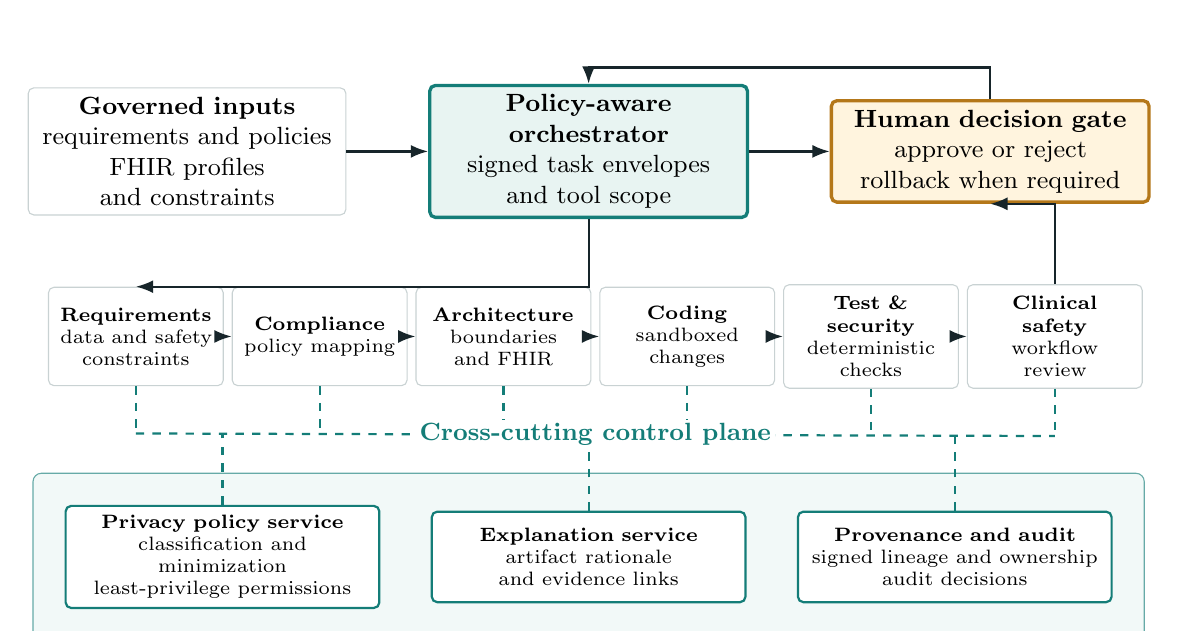
\begin{tikzpicture}[
  input/.style={draw=grayline,fill=white,rounded corners=2pt,text width=3.8cm,
    minimum height=1.15cm,align=center,font=\small},
  orchestrator/.style={draw=teal,fill=teallight,very thick,rounded corners=2pt,
    text width=3.8cm,minimum height=1.15cm,align=center,font=\small},
  human/.style={draw=gold,fill=goldlight,very thick,rounded corners=2pt,
    text width=3.8cm,minimum height=1.15cm,align=center,font=\small},
  agent/.style={draw=grayline,fill=white,rounded corners=2pt,text width=1.92cm,
    minimum height=1.25cm,align=center,font=\fontsize{7}{8}\selectfont,inner sep=1.5mm},
  service/.style={draw=teal,fill=white,thick,rounded corners=2pt,text width=3.75cm,
    minimum height=1.15cm,align=center,font=\scriptsize},
  arrow/.style={-{Latex[length=2.2mm]},thick,draw=ink},
  controlbus/.style={draw=teal,thick,dashed},
  boundary/.style={draw=teal!65,fill=teallight!55,rounded corners=3pt,inner sep=4mm}
]
\node[input] (inputs) at (-5.1,0)
  {\textbf{Governed inputs}\\requirements and policies\\FHIR profiles and constraints};
\node[orchestrator] (orch) at (0,0)
  {\textbf{Policy-aware orchestrator}\\signed task envelopes and tool scope};
\node[human] (gate) at (5.1,0)
  {\textbf{Human decision gate}\\approve or reject\\rollback when required};

\node[agent] (req) at (-5.75,-2.35) {\textbf{Requirements}\\data and safety constraints};
\node[agent,right=1mm of req] (comp) {\textbf{Compliance}\\policy mapping};
\node[agent,right=1mm of comp] (arch) {\textbf{Architecture}\\boundaries and FHIR};
\node[agent,right=1mm of arch] (code) {\textbf{Coding}\\sandboxed changes};
\node[agent,right=1mm of code] (test) {\textbf{Test \& security}\\deterministic checks};
\node[agent,right=1mm of test] (safety) {\textbf{Clinical safety}\\workflow review};

\node[service] (privacy) at (-4.65,-5.15)
  {\textbf{Privacy policy service}\\classification and minimization\\least-privilege permissions};
\node[service] (explain) at (0,-5.15)
  {\textbf{Explanation service}\\artifact rationale\\and evidence links};
\node[service] (prov) at (4.65,-5.15)
  {\textbf{Provenance and audit}\\signed lineage and ownership\\audit decisions};

\begin{scope}[on background layer]
  \node[boundary,fit=(privacy)(explain)(prov)] {};
\end{scope}

\draw[arrow] (inputs) -- (orch);
\draw[arrow] (orch) -- (gate);
\draw[arrow] (orch.south) |- (req.north);
\draw[arrow] (req) -- (comp);
\draw[arrow] (comp) -- (arch);
\draw[arrow] (arch) -- (code);
\draw[arrow] (code) -- (test);
\draw[arrow] (test) -- (safety);
\draw[arrow] (safety.north) |- (gate.south);
\draw[arrow] (gate.north) -- ++(0,4mm) -| (orch.north);

\coordinate (busleft) at ($(req.south)+(0,-6mm)$);
\coordinate (busright) at ($(safety.south)+(0,-6mm)$);
\draw[controlbus] (busleft) -- (busright);
\foreach \x in {req,comp,arch,code,test,safety}
  \draw[controlbus] (\x.south) -- (\x.south |- busleft);
\foreach \x in {privacy,explain,prov}
  \draw[controlbus] (\x.north) -- (\x.north |- busleft);
\node[fill=white,inner sep=1.5pt,font=\bfseries\small,text=teal]
  at ($(busleft)!0.5!(busright)$) {Cross-cutting control plane};
\end{tikzpicture}
\caption{Candidate governed multi-agent framework for healthcare software development. Control services apply across the lifecycle rather than acting as a final review step.}
\label{fig:framework}
\end{figure}

The Requirements Agent extracts functional behavior, stakeholders, data classes, consent assumptions, safety constraints, and acceptance criteria. The Compliance Agent maps these items to supplied policy rules and marks unresolved jurisdictional questions. It does not declare legal compliance. The Architecture Agent proposes services, data flows, trust boundaries, FHIR resources, and failure behavior. The Coding Agent works only from approved requirements and architecture.

The Test and Security Agent generates unit, integration, authorization, audit, privacy, FHIR, and adversarial tests. Deterministic scanners and validators supplement its judgment. The Clinical Safety Agent reviews whether the software could bypass professional review, present unsupported claims, mishandle uncertainty, or alter a clinical workflow without approval. The Human Gatekeeper owns high-risk transitions.

Three cross-cutting services apply at every stage. The Privacy Control classifies inputs, filters context, restricts tools, and checks outputs. The Explanation Service builds structured explanations from recorded inputs and evidence. The Provenance Service signs task envelopes and links requirements, actions, artifacts, test results, reviews, and approvals. These services should not rely on the same generative model that creates the code.

\subsection{Phase 4: prototype and experimental tasks}

The prototype will use synthetic FHIR data only. A compact test suite can include patient registration, consent-aware record retrieval, appointment scheduling, medication-list update, and audit-event generation. Each task should include functional requirements, a FHIR profile or constraint set, access roles, privacy rules, acceptance tests, and one adversarial variation.

The framework will run inside a sandboxed repository with no production credentials. Agents receive the minimum tools needed for their role. Generated services should expose a small API, store no real health data, and produce reproducible build and test artifacts. Model versions, prompts, parameters, tools, and seeds will be recorded.

Each task will run several times to capture stochastic variation. Failed runs remain part of the dataset. Removing them would overstate reliability. The experiment will preserve intermediate artifacts so researchers can distinguish a planning failure from a coding, testing, or approval failure.

\subsection{Phase 5: comparative and ablation evaluation}

Three main conditions test the value of governance. Baseline A uses one development agent with the same task and tool budget. Baseline B uses specialist agents but removes dedicated privacy, explanation, provenance, and human-gate controls. Condition C uses the complete framework. The task set, model family, token budget, and validator suite should remain as constant as practical.

An ablation study removes one cross-cutting control at a time from Condition C. Privacy ablation measures leakage and over-collection. Explanation ablation measures reviewer understanding and evidence alignment. Provenance ablation measures trace completeness and fault localization. Human-gate ablation measures unsafe transition rate. These tests show whether a component adds measurable value instead of architectural complexity alone.

Adversarial evaluation injects prompt instructions hidden in requirements, poisoned messages from a simulated agent, false test-success claims, excessive data requests, malformed FHIR resources, stale consent, unauthorized role changes, and a deployment request without approval. The system should block, quarantine, or escalate each case and preserve evidence for diagnosis.

\subsection{Metrics}

Correctness metrics include build success, unit and integration test pass rate, task completion, defect count, and requirement coverage. Interoperability metrics include FHIR validator pass rate, profile conformance, terminology checks, and negative-test behavior. Security metrics include static findings, authorization bypasses, secret exposure, and adversarial attack success.

Privacy metrics include exposure of sensitive fields, unnecessary fields supplied to agents, canary leakage, policy violations, memory persistence after task completion, and retention-rule failures. A privacy result should report both frequency and severity. One disclosure of a high-sensitivity field may matter more than several low-impact formatting errors.

Explanation metrics include schema completeness, correct links to requirements and evidence, contradiction rate, unsupported-claim rate, and reviewer usefulness. Faithfulness will be assessed against recorded actions and tool results, not hidden model reasoning. Reviewers should answer whether they can identify what changed, why, which constraints applied, what evidence passed, and what risk remains.

Provenance metrics include the percentage of artifacts with complete ancestry, signature verification, orphaned actions, and time to locate the source of an injected fault. Governance metrics include unsafe transitions blocked, false blocks, review time, rejection quality, and successful rollback. Cost metrics include runtime, model calls, token use, and human effort.

The analysis should report distributions and confidence intervals where repeated runs permit them. It should avoid collapsing all outcomes into one score. A framework can improve privacy while increasing review time; that trade-off should remain visible.

\subsection{Validity and ethics}

Construct validity depends on whether the metrics represent privacy, explanation, safety, and governance. The study will publish operational definitions and use deterministic checks where possible. Human explanation ratings require a rubric, training examples, and inter-rater agreement. Internal validity requires comparable models, tools, and budgets across conditions. Repeated runs and preserved traces will help identify random variation.

External validity will remain limited because synthetic FHIR tasks cannot reproduce institutional systems, clinician workload, or patient consequences. The study should claim engineering evidence in a controlled setting, not clinical effectiveness. Later work can add expert review and partner-defined scenarios after governance approval.

The research avoids real patient data. Synthetic records must still avoid copying identifiable examples. Clinicians, privacy specialists, software engineers, and potential users should review requirements and explanation formats. Their involvement does not turn the prototype into a certified medical device or prove regulatory compliance.

Automation bias is an experimental concern as well as a deployment concern. Review interfaces should avoid presenting agent confidence as authority. They should show failed tests, unresolved assumptions, missing evidence, and alternative decisions. Reviewers need a practical rejection path and should not be penalized for stopping a run.

\section{Discussion}

The corpus supports a focused contribution. Healthcare MAS research already supplies role specialization, secure communication, access control, modular EHR interaction, audit logging, and a mature account of ethical risks. It does not integrate those elements around the software-development artifact. The proposed framework uses that missing unit to connect privacy, explanation, provenance, and human approval.

The contribution should remain narrower than ``autonomous healthcare development.'' A credible first prototype can automate bounded tasks inside a sandbox and require approval before high-risk transitions. It should show that control services improve measurable outcomes. Expanding autonomy before that evidence exists would reproduce the validation weakness reported across the literature.

The framework also should resist compliance theater. Mapping a requirement to a regulation label does not prove compliance. A Compliance Agent can identify controls, missing information, and review obligations. Legal and institutional owners must decide whether the implementation satisfies applicable rules. The thesis should describe technical alignment and evidence generation, not certification.

Explainability should follow the same discipline. A generated paragraph that sounds plausible is not an explanation unless it matches the recorded action and evidence. Structured artifact records allow validators and reviewers to test that match. This approach also limits disclosure of sensitive chain-of-thought content.

The proposed baseline and ablation design addresses a weakness in many agent frameworks: they add roles without measuring whether each role helps. Comparing one agent, uncontrolled specialist agents, and the governed framework can isolate the benefit of coordination and controls. Ablation can expose controls that add cost without reducing risk.

The study's largest limitation remains its purposive scope. Recent publications dominate, several reviews cover overlapping literature, and the technical contributions provide limited empirical validation. Software engineering, medical-device lifecycle standards, and agentic coding research were not primary search domains. The research-gap claims therefore need later confirmation through a targeted systematic search.

Despite that limit, the evidence is sufficient for a defensible thesis direction. Multiple source types converge on weak validation, privacy risk, explainability needs, interoperability barriers, and blurred responsibility. The proposed methodology turns those recurring concerns into testable engineering requirements rather than repeating them as general principles.

\section{Conclusion}

This scoping study synthesized selected research on healthcare multi-agent systems, privacy, explainability, interoperability, governance, and validation. The literature shows that healthcare MAS can coordinate specialized roles in operations, decision support, critical care, secure communication, and EHR interaction. It also provides concrete privacy mechanisms through access control, encryption, group-key agreement, controlled FHIR operations, and audit logging. Explainability, governance, and real-world validation remain less mature.

No included paper implements a governed multi-agent lifecycle that produces healthcare software artifacts. No paper combines artifact-level explanations, development-data privacy, end-to-end provenance, executable interoperability constraints, risk-based human gates, and a multi-dimensional evaluation. These corpus-supported gaps define the proposed contribution.

The recommended research method uses Design Science Research to build and evaluate a bounded framework with specialized lifecycle agents and cross-cutting privacy, explanation, and provenance services. The experiment uses synthetic FHIR tasks, three architecture conditions, component ablations, deterministic validators, human review, and adversarial failures. The study will report correctness, privacy, interoperability, explanation, provenance, security, cost, and review burden separately.

The resulting research should be judged by evidence of control, not by the amount of autonomy it demonstrates. A useful framework will show which agent acted, which data and policy it used, why an artifact changed, which tests support it, who approved the risk, and how the system can stop or recover when those conditions fail.

\clearpage
\bibliographystyle{IEEEtran}
\bibliography{references}

\end{document}
